\section{Actor Grafik Legende}\label{actor:diagram:description}
Um den Ablauf in einem Actor-System besser zu verstehen bittet sich die visuelle Darstellung in Form von Diagrammen eines Actors oder eines Actor-Systems an. In den Werken \cite{kuhn2017reactive} und \cite{Vernon2015ReactiveAkka} wurde eine einheitliche, grafische Notation für das Actor Model vorgeschlagen, welche auch für diese Arbeit herangezogen wird. Im folgenden nun eine kleine Einführung in diese Notation, welche die für diese Arbeit notwendigen Notationen darstellt und deshalb kein Anspruch auf Vollständigkeit stellt.\\
\subsection{Actors darstellen}
    Ein einzelner Actor wird als Kreis dargestellt, innerhalb dieses Kreises steht der Name des Actors. In Abbildung~\ref{fig:actor:diagram:longLiveActor} wird ein Actor dargestellt welcher persistent existiert, im gegensatz dazu steht ein Actor welcher nur für eine kurze Zeit existiert dieser wird mit gestrichelter Linien, siehe Abbildung~\ref{fig:actor:diagram:shortLiveActor}, dargestellt. Ein Actor welcher nur für kurze Zeit existiert, wird meist verwendet um eine einzelne spezielle Nachricht abzuarbeiten.
\begin{figure}
    \centering
    \begin{minipage}{.5\textwidth}
      \centering
      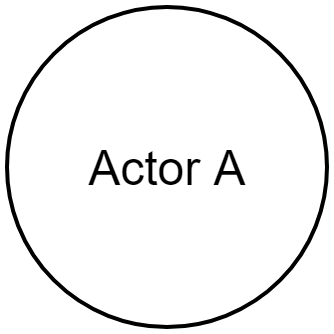
\includegraphics[width=.5\linewidth]{gfx/actor/longLiveActor}
      \captionof{figure}{Ein einfacher Actor.}
      \label{fig:test1}
    \end{minipage}%
    \begin{minipage}{.5\textwidth}
      \centering
      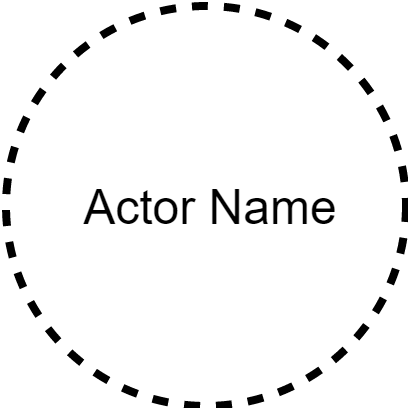
\includegraphics[width=.5\linewidth]{gfx/actor/shortLiveActor}
      \captionof{figure}{Ein Actor welcher direkt nach der Abarbeitung einer Nachricht wieder zerstört wird.}
      \label{fig:test2}
    \end{minipage}
    \end{figure}  

\subsection{Nachrichten erstellen}
Das erstellen einer Nachricht durch den Actor {A} sowie die Zustellung durch den Actor {A} and den Actor {B} wird in Abbildung~\ref{fig:actor:diagram:simpleCreateAndSendMessage} abgebildet. Wichtig ist hier, dass der Actor {A} nicht nur die Nachricht sendet, sondern sie auch erstellt!
\begin{figure}
    \centering
    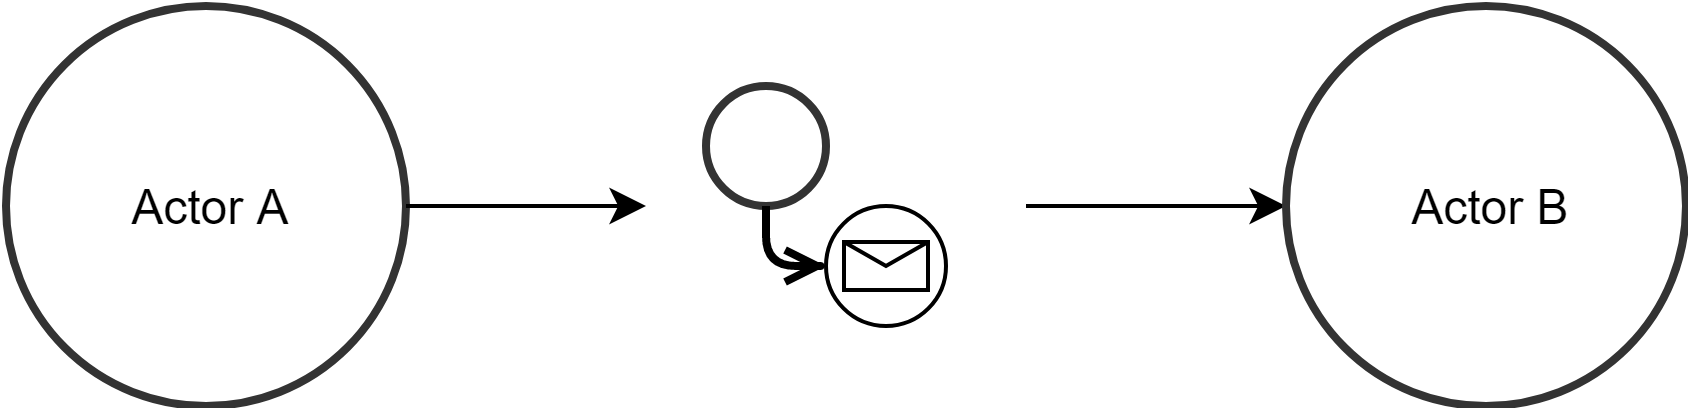
\includegraphics[width=\linewidth]{gfx/actor/simpleCreateAndSendMessage}
    \caption{Actor {A} erstellt eine neue Nachricht und sendet sie an Actor {B}.}
    \label{fig:actor:diagram:simpleCreateAndSendMessage}
\end{figure}

\subsection{Actors erstellen}
Das erstellen von Actoren durch einen Actor wird durch zwei kreise abgebildet. In Abbildung~\ref{fig:actor:diagram:childActorCreation} erstellt der {Parent}-Actor einen neuen Actor, den sogenannten {Child}-Actor.
\begin{figure}
    \centering
    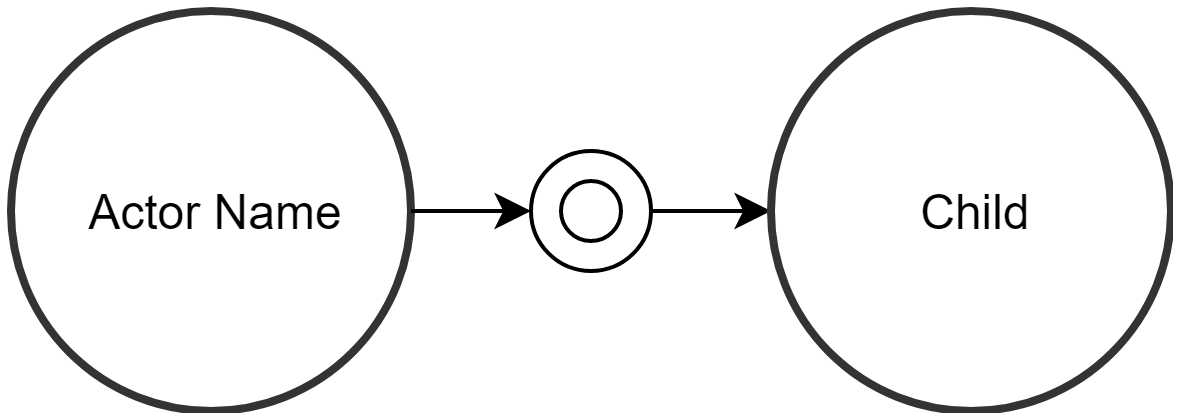
\includegraphics[width=\linewidth]{gfx/actor/childActorCreation}
    \caption{Ein Actor erstellt einen neuen Actor}
    \label{fig:actor:diagram:childActorCreation}
\end{figure}

\subsection{Darstellung eines Ablaufes}
Um einen konkreten Ablauf eines Actors darstellen zu können, benötigt man die darstellung der Nachrichteneingangsreihenfolge. Diese wird von \cite{kuhn2017reactive} und \cite{Vernon2015ReactiveAkka} als Linie dargestellt auf welcher sich Kreise befinden. Die abarbeitung wird von oben nach unten dargestellt. In Abbildung~\ref{fig:actor:diagram:asynchronMessageReceivment} bekommt der Actor zwei Nachrichten zugesendet, und sendet eine Nachricht dazwischen ab. Durch diese Abbildung ist es möglich, sequentielle Abläufe darzustellen
\begin{figure}
    \centering
    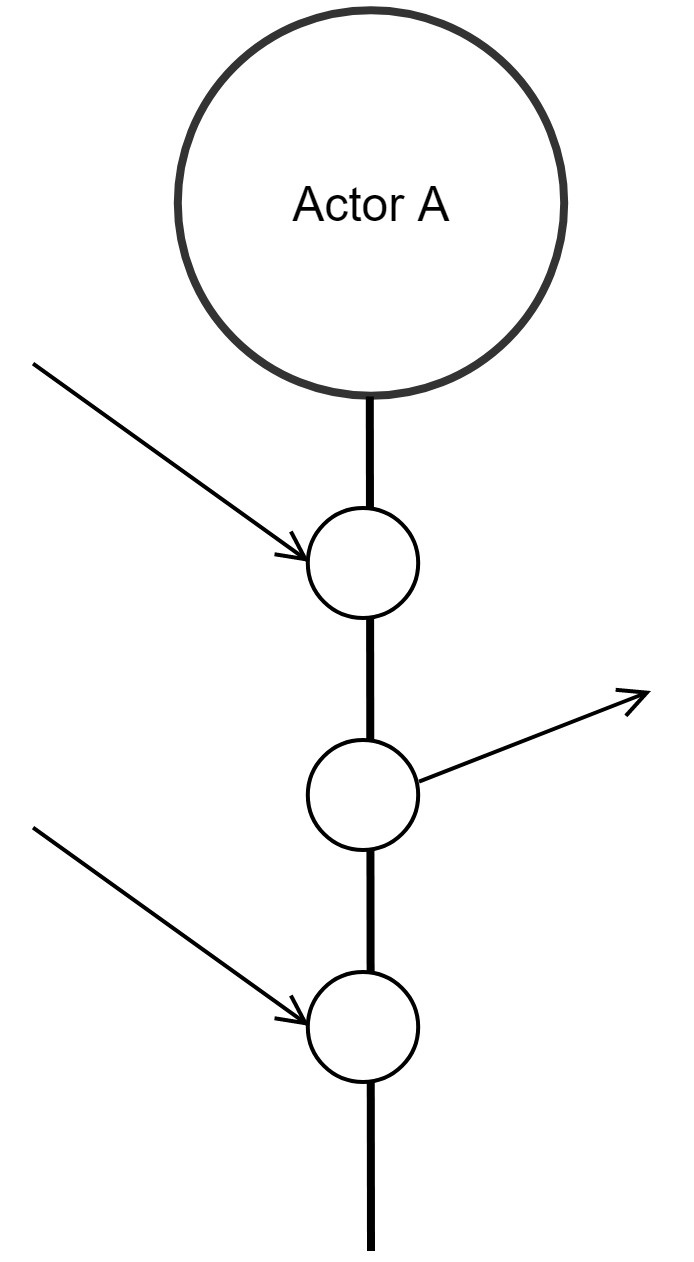
\includegraphics[height=6cm]{gfx/actor/actorAsynchMessgeFlow}
    \caption{Asynchroner Ablauf eines Actors.}
    \label{fig:actor:diagram:asynchronMessageReceivment}
\end{figure}